
% this file is called up by thesis.tex
% content in this file will be fed into the main document

%: ----------------------- introduction file header -----------------------
% the code below specifies where the figures are stored
\graphicspath{{3/figures/}}

\chapter{Deep Learning}
\label{chp:deep_learning}


Deep learning descends from a long and, at times, rocky history of artificial intelligence, information theory, and computer science.
% TODO: There is a sentence / thought missing here.
The goals of this chapter are two-fold:
Section \ref{sec:background} first offers a concise summary of the history of deep learning in three parts, detailing the origins, critical advances, and current state of the art of neural networks.
Afterwards, a formal treatment of deep learning is addressed in three parts:
Section \ref{subsec:architectures} introduces the architectural components of deep networks;
Section \ref{subsec:learning} introduces the process of automatic learning, covering the design of loss functions and basic theory of gradient-based optimization;
and Section \ref{subsec:tricks} outlines various tricks of the trade and other practical considerations in the use of deep learning.
Finally, the concepts introduced in this chapter are briefly summarized in Section \ref{sec:deep_summary}.


\section{A Brief History of Neural Networks}
\label{sec:background}
Despite the recent wave of interest and excitement surrounding it, the core principles of deep learning were originally devised halfway through the 20th century, grounded in mathematics established even earlier.
As a direct descendant of neural networks ---computational models with an ambitious moniker burdened by a tumultuous past--- the very mention of deep learning often ellicts several warranted, if suspicious, questions: What's the difference? What's changed? Why do they suddenly work \emph{now}?
Thus, before diving into a formal review of the deep learning and its various components, it is worthwhile to contextualize the research trajectory that has led to today.


\subsection{Origins (pre-1980)}
\label{subsec:origins}

For Western Europe and those in its sphere of influence, the Age of Enlightenment marked a golden era of human knowledge, consisting of great advances in many diverse fields, such as mathematics, philosophy, and the physical sciences.
Long had humanity contemplated the notions of consciousness and reasoning, but here brilliant thinkers began to return to and explore these concepts with resolve.
From the efforts of scholars like Gottfried Leibnitz, Thomas Hobbes, and George Boole, formal logic blossomed into its own mathematical discipline.
In doing so, it became possible to symbolically express the act of reasoning, whereby rational thought could be described by a system of equations to be transformed or even solved.

It was this critical development ---the idea of logical computation--- that encouraged subsequent generations to speculate on the apparent feasibility of artificial intelligence.
And, coinciding with the advent of electricity in the 20th century, mathematicians, philosophers, and scientists of the modern era sought to create machines that could \emph{think}.
While the space of relevant contributions is too great to enumerate here, there were a handful of breakthroughs that would prove integral to the field of computer science.
In 1936, Alan Turing devised the concept of a ``universal machine'', which would lead to the proof that a system of binary states, e.g. true and false, could be used to perform \emph{any} mathematical operation \cite{Turing1936Computable}.
Only shortly thereafter, Claude Shannon demonstrated in his \emph{master's} thesis that Boolean logic could be implemented in electrical circuits via switches and relays, forming the basis of the modern computer \cite{Shannon1938Symbolic}.
Shortly thereafter, in 1943, McCulloch and Pitts constructed the first artificial neuron, a simple computational model inspired by discoveries in neuroscience \cite{Mcculloch1943Logical}.
By coarse analogy to biology, an artificial neuron ``fires'' when a weighted combination of its inputs eclipse a given threshold:

\begin{align*}
  f(\mathbf{x}~|~\mathbf{w}) = h(\mathbf{w}^T~\cdot~\mathbf{x})\\
  h(y) = \left\{
    \begin{array}{ll}
      1 : y \ge 0\\
      0 : y < 0\\
    \end{array}
  \right.
\label{eq:perceptron}
\end{align*}

\noindent Importantly,
%as shown in Figure \ref{fig:neuron_logic},
it was demonstrated that such a model could be used to reproduce Boolean operations, such as AND or OR.
Given the clear application to the field of computational logic, artificial neurons only further encouraged the pursuit of artificially ``intelligent'' machines.

% Perceptron!
On its own, an artificial neuron is only a general processing structure, and the parameters it takes will specify the precise behavior of the model.
Arriving at these parameters, however, was nontrivial and required manual derivation.
Thus, in 1958, Frank Rosenblatt's invention of the \emph{Perceptron} algorithm significantly altered how artificial neurons were conceived \cite{Rosenblatt1958Perceptron}.
Building upon the work of McCulloch and Pitts, the algorithm, given in \Cref{alg:perceptron}, offered an automated method of ``learning'' the parameters necessary to achieve binary classification over a collection of data:

\begin{algorithm}[H]
\caption{Find the optimal parameters for a Perceptron over a collection of data.}
\label{alg:perceptron}
\small
\begin{algorithmic}[1]
\Procedure{FitPerceptron}{$\mathbf{x}, \mathbf{y}, \eta, n_{max}$}
    \State $\mathbf{w} \gets \mathbf{0}_{(D + 1, 2)}$
    \State $\mathbf{e} \gets \mathbf{1}_{N}$
    \State $n \gets 1$
    \While {$|\mathbf{e}| > 0$ \textbf{and} $n < n_{max}$}
        \State $\mathbf{z} \gets f(\mathbf{x} | \mathbf{w})$
        \State $\mathbf{e} \gets \mathbf{z} - \mathbf{y}$
        \State $\mathbf{w} \gets \mathbf{w} + \eta (\mathbf{e}^T \cdot \mathbf{x})^T$
        \State $n \gets n + 1$
    \EndWhile
    \State Return $\mathbf{w}$
\EndProcedure
\end{algorithmic}
\end{algorithm}

\noindent The perceptron algorithm requires four inputs:
a matrix of observations, $\mathbf{x} \in \mathcal{R}^{N\times D}$, corresponding to $N$ samples with $D$ dimensions;
a vector of binary class assignments, $\mathbf{y}$, in the set $\{0, 1\}$;
a learning rate parameter, $\eta$;
and an iteration limit, $n_{max}$.
Initializing the algorithm, the weights, $\mathbf{w}$, are set to a matrix of zeros, shaped $(D + 1, 2)$, an error, $\mathbf{e}$, is set to a vector of ones, and the iteration counter, $n$, starts from 1.
Then, in an iterative manner, binary outputs, $\mathbf{z}$, are computed from the perceptron function, $f()$,
% given in Eq. \ref{eq:perceptron},
the error is computed as the difference between class predictions and targets, and the weights are updated with a scaled version of the incorrectly classified inputs.
Note that the error vector, $\mathbf{e}$ is only non-zero where the predicted values are wrong, and thus the algorithm naturally terminates when all datapoints are classified correctly.
Alternatively, execution is halted once a fixed number of iterations is reached.
An example of a perceptron's stopping condition is given in Figure \ref{fig:linsep}.
Here, a perceptron has separated two classes of data, drawn from different Gaussian distributions.
As the algorithm proceeds, the total error decreases until a decision boundary is found that correctly classifies the observed data.

\begin{figure}
\begin{centering}
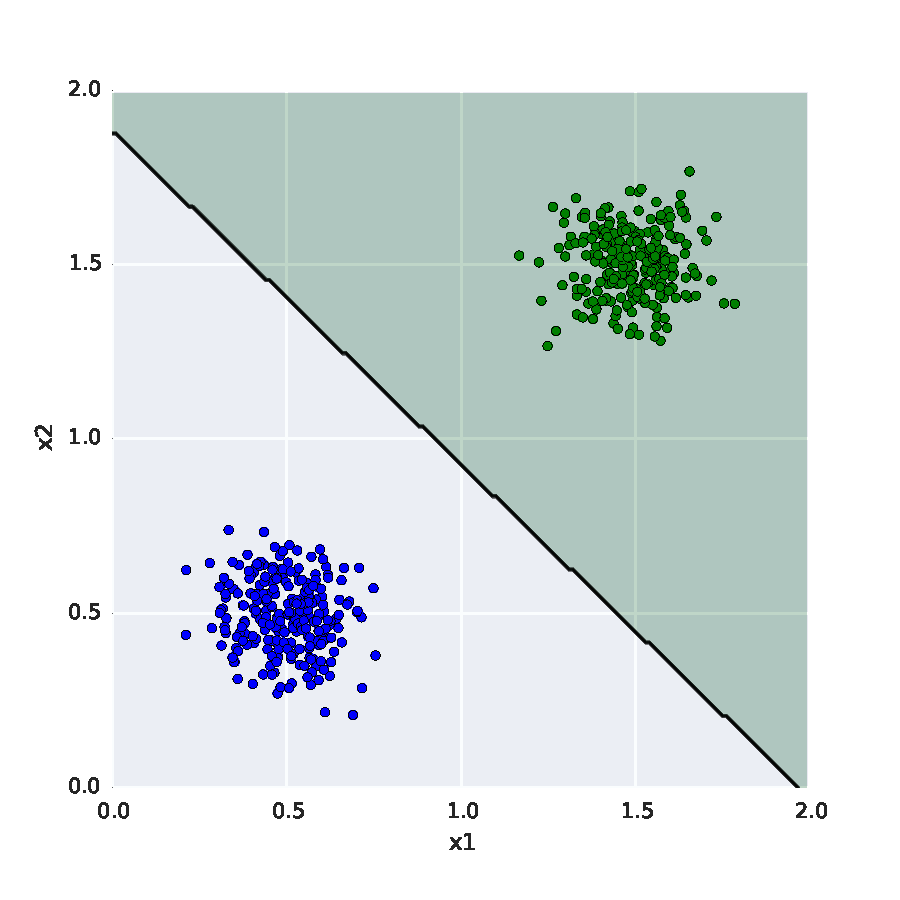
\includegraphics[width=0.6\textwidth]{linsep}
\caption{Linearly separable data classified by a trained perceptron.}
\label{fig:linsep}
\end{centering}
\end{figure}

% Promise and limitations
Once implemented in hardware, using a slew of potentiometers, motors, and photocells, Rosenblatt's' ``Mark I Perceptron'' drew considerable attention from the press and the research community alike.
The \emph{New York Times} was quick to publish ambitious claims as to the promise this breakthrough held for artificial intelligence and the speed at which subsequent advances would be realized, much to the eventual chagrin of the AI community \cite{Olazaran1996Sociological}.
However, the Perceptron was not without limitations nor critics.
In their book, \emph{Perceptrons}, published in 1969, Minsky and Papert demonstrated that the model is rather limited in the kinds of behavior it can actually achieve \cite{Minsky1969Perceptrons}.
For example, perceptrons are unable to reproduce the logic of an exclusive-or (XOR), and thus can only classify \emph{linearly separable} data, the condition where a single straight line can be drawn between two classes.
% This scenario is illustrated in Figure \ref{fig:mlp_ftw}, where no single line can be draw to correctly classify the data.

% Multilayer Perceptrons
This was a critical limitation for researchers in the field of neural computation; if a perceptron could not perform basic logic operations, how could it be expected to reason?
The answer, as it would turn out, could be found by transforming how the XOR function is expressed symbolically.
Rearranging terms, an equivalent function can be rewritten as the disjunction (OR) of two complementary conjunctions (AND):

\begin{equation}
\label{eq:xor}
p \oplus q = (p \wedge \neg q) \vee (\neg p \wedge q)
\end{equation}

\noindent While it is true that a single Perceptron cannot achieve the XOR operation directly, a combination of \emph{three} can: two are used to perform each AND operation and corresponding negation, while a third performs the OR operation.
Considering the scenario in Figure \ref{fig:mlp_ftw}, this condition can now be easily separated by a \emph{multilayer} perceptron (MLP).
Therefore, arbitrarily complex functions could be obtained by cascading simpler non-linear operations, leading to a class of functions that would come to be known as \emph{neural networks}.
These models are so versatile, in fact, it would later be shown by the \emph{universal approximation theorem} that a neural network is actually able to model \emph{any} continuous function, within some error tolerance \cite{Cybenko1989Approximation, Hornik1991Approximation}.

\begin{figure}
\begin{centering}
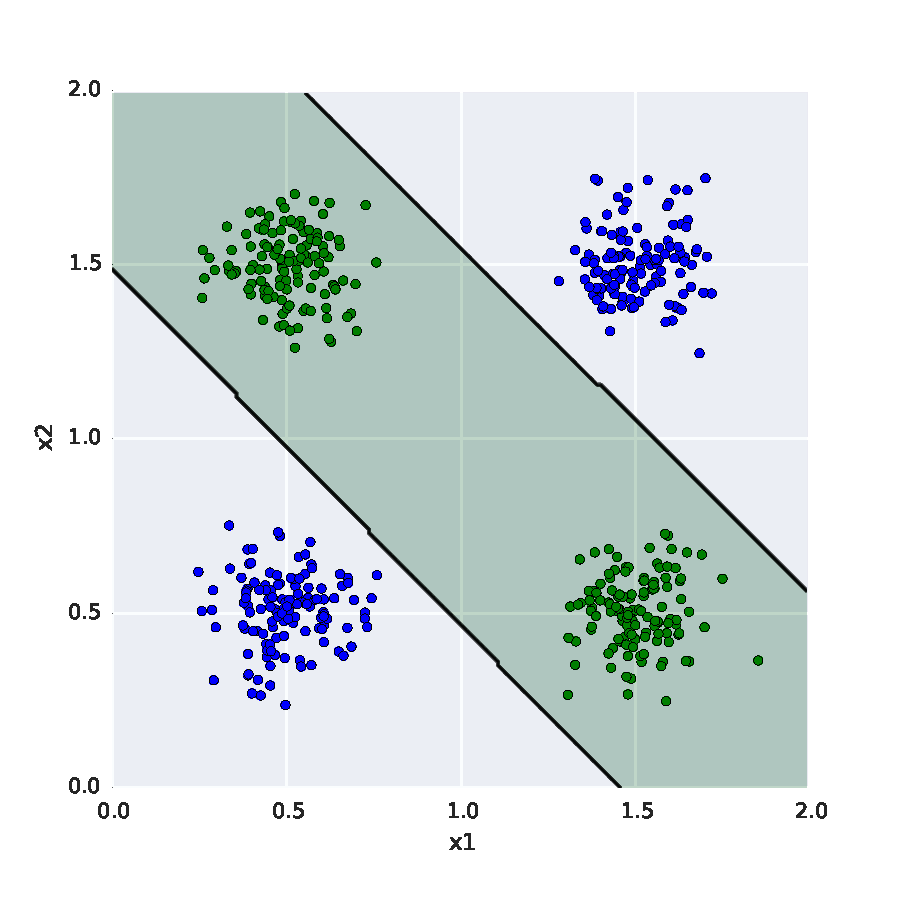
\includegraphics[width=0.6\textwidth]{mlp_ftw}
\caption{Demonstration of the decision boundaries for a \emph{multi-layer} perceptron.}
\label{fig:mlp_ftw}
\end{centering}
\end{figure}

% Other problems
Despite this promising observation, neural network research languished through the closing decades of the 20th century, suffering a considerable drop in funding support and, as a result, interest.
While the representational power of multilayer perceptrons was recognized early on, it became popular opinion that these models could not be used to solve complex problems.
In addition to theoretical skepticism, those who continued to pursue neural network research were also faced with an array of practical challenges.
Neural networks were prone to over-fitting, extremely slow to train, and difficult to use with more than a few layers.
% Ahead of the times
% Theory outpaced technological capacity. Over-hyped
Independently, these issues might merely have been viewed as common research obstacles.
However, coupled with the failed promises of early progress, such difficulties would malign the pursuit of neural network research for some time.
% This resulted in what is affectionately known as one of the ``AI winter'', things got bad.


\subsection{Scientific Milestones (1980--2010)}
\label{sec:advances}

In the face of widespread pessimism toward neural computing, some researchers would persevere through this ``AI Winter''.
Over the course of thirty some years, these diligent efforts would result in crucial breakthroughs that, in combination with the steady churn of technological progress, would fundamentally change the landscape of neural network research.
While no one facet can truly be credited with reviving the field, each would play an integral role in helping the research community again warm up to neural networks.

\subsubsection{Efficient Error Backpropagation}
\label{subsec:sgd}

% Back-propagation of errors
Via the perceptron algorithm, a machine effectively ``learns'' to classify data by finding parameters that optimize a given objective function.
This learning strategy must be modified in the multilayer case, as it is not possible to directly update the parameters through the heaviside, or unit step, function.
Early researchers noted that if the discontinuous activation function is replaced with a logistic, or sigmoid, the composite multilayer network is \emph{differentiable}.
Thus, as will be discussed in more detail in Section \ref{subsubsec:numopt}, it is possible to use this gradient information to optimize the parameters of a network given an objective fitness measure, effectively \emph{back-propagating} error through the network \cite{Hinton1986Learning}.

% Issues of gradient descent
% This is a critical Once you can differentiate the network, gradient methods can be used to optimize the parameters.
This approach was not without its deficiencies, however.
First and foremost, the error term was typically computed over the entire dataset, which often proved computationally expensive for sufficiently large collections.
Additionally, early efforts found this particular approach often resulted in poor answers, and struggled to update parameters of networks with many layers.
%Stochastic Gradient Descent
In time, a \emph{stochastic} variant of this algorithm was shown to be far more efficient, and even circumvented some of these issues \cite{LeCun1998Efficient}.
Whereas conventional optimization occurs over an entire collection of datapoints, this efficient version randomly subsamples the training set and computes the error term over fewer datapoints.
Though the error estimate is much noisier, the strategy is still effective, significantly faster, and may even be less susceptible to bad parameters as a result.

\subsubsection{Convolutional Neural Networks}
\label{subsec:convnets}

% Fully connected networks, bleh; sensitive to translation and scale
% TODO: Needs a better context sentence

Though equal parts remarkable and encouraging, the universal approximation theorem has significant practical limitations.
First, the theorem only holds for a sufficiently, and perhaps infinitely, wide network.
Additionally, it says nothing about how one might parameterize such a function in order to achieve some desired behavior.
Thus, despite such overwhelming promise, early neural networks often resulted in poor approximations of the functions being modeled, because the flexibility of the model vastly surpassed the amount of data available to train it.
This flexibility was apparent in computer vision tasks, as multilayer perceptrons struggled to cope with simple homographic deformations, such as translation, scaling, or rotation.

% Visual cortex, neocognitron
Natural vision systems, on the other hand, are quite robust to these kinds of variation, and, as before, researchers looked to biology for inspiration in modeling these processes.
One particularly insightful study was that of Hubel and Wiesel in 1959, who experimented on the neural behavior of the feline visual cortex \cite{Hubel1959Receptive}.
By presenting visual stimuli while probing the brain with electrodes, they discovered two different kinds of neurons ---simple cells and complex cells--- organized hierarchically.
Experimental results indicated that the former is responsible for local feature extraction, while the latter combines the inputs of simple cells to absorb small amounts of variation in the observed stimuli.

% ConvNets, LeNet5, handwritten digits
These ideas were first incorporated in the Neocognitron \cite{Fukushima1988Neocognitron}, and later realized successfully as a convolutional neural network for shape recognition and handwritten digit classification \cite{LeCun1998Gradient}, offering three key design features.
\emph{Local receptive fields} produce outputs over a small neighborhood of input features, exploiting the observation that nearby pixel values tend to be highly correlated.
Smaller receptive fields result in models that require a fewer number of parameters, thus reducing the overall size of the model and the amount of data needed to train it.
Applying local receptive fields as a convolution results in effectively sharing the weights over all positions in an image.
Thus \emph{weight sharing} reduces the number of parameters even further, while allowing the network to identify features regardless of position in an image.
Finally, \emph{pooling} reduces small number of inputs to a single value by a given function, such as the mean or max, introducing not only shift but a small amount of scale and rotation invariance.
Taken together, these advantageous attributes directly resolved many of the issues plaguing multilayer perceptrons, and proved to be the most successful instance of neural computing for nearly two decades.


% Theory preceded data
\subsubsection{Proliferation of Digital Data}
\label{subsec:perceptrons}

% Early data
Given the ubiquity of digital information in the modern era, it is easy to forget that neural networks were first developed in a considerably different day and age.
The very existence of digital audio and images, for example, did not become commonplace until the end of the 20th century.
Even then, these signals were costly to create, cumbersome to process, and generally difficult to distribute.
Furthermore, once obtained, the process of annotating this information for use in supervised learning requires a great deal of time and effort.
Thus, in the vein of speech recognition or computer vision for example, machine perception research was forced to work with small datasets as a result.
Given the versatility of neural networks to model complex data, it was typically trivial to over-fit these small training, while failing to generalize to new data.
Neural networks developed the reputation of being ``data hungry'', requiring a large amount of training data in order to do anything useful in practice.

% Labeled datasets grew, intentionally or otherwise
While this was, and in some cases still is, a valid concern for neural networks, the problem of data scarcity is far less of an issue now.
For many well worn tasks, researchers have had ample time to curate massive labeled datasets.
In the late 1980s, LeCun et al. oversaw the development of a handwritten digit dataset, comprised of 60k 28x28 pixel images \cite{LeCun1998MNIST};
for comparison, the ImageNet dataset consists of millions of tagged, high resolution images \cite{Deng2009Imagenet}.
Similar efforts have been undertaken in the fields of speech recognition \cite{Fisher1986TIMIT}, face recognition \cite{Huang2007Labeled}, or natural language processing \cite{Lewis2004RCV1}, to name only a few.
Additionally, given the rise of the Internet, it became possible to leverage a variety of information sources to obtain labeled data, such as user-generated content, via Last.fm\footnote{\url{http://www.last.fm/}} or Twitter\footnote{\url{http://www.twitter.com/}}, weak feedback signals, e.g. Pandora Radio\footnote{\url{http://www.pandora.com/}}, or even as a means of distributing the annotation effort \cite{Von2003Captcha}.
Combined, the range of information available for large-scale supervised learning grew considerably, diminishing the issues posed by data-hungry algorithms.

% unlabeled data has uses too
As a by-product of the global transition to the digital realm though, an even larger portion of \emph{unlabeled} data was at the disposal of machine learning researchers.
Coupling the easy availability of digital information with the idea that ``the human brain isn't \emph{really} supervised'', much effort was invested in the space of \emph{unsupervised} learning algorithms. %, i.e. learning from unlabeled data.
Finally, in 2006, one such method, referred as \emph{contrastive divergence}, was able to successfully exploit unlabeled data to improve the performance of a neural network \cite{Hinton2006Fast}.
Using a cascade of undirected models, known as a Restricted Boltzmann machine (RBM), a neural network was trained in a greedy, layer-wise manner to reproduce realistic data.
After this process of learning how real data behaves, the model could be ``fine-tuned'' with a smaller amount of labeled data to realize impressive, state of the art performance.
Referred to as ``pre-training'', learning on unsupervised data allowed the model to discover parameters closer to a good final solution.
Though later discoveries would demonstrate pre-training to be unnecessary under certain conditions \cite{Zeiler2013Rectified}, this breakthrough was perhaps the first to forcefully recapture the attention of the machine learning community.

% Subsequently, similar unsupervised approaches
%  called an autoencoder \cite{Vincent2010}, or ---an alternative interpretation from another research team--- Predictive Sparse Decomposition \cite{Ranzato2007}, incorporates roughly the same principles with deterministic interpretation of these concepts.
% In either view of the parameter optimization problem, learning algorithms now exist that can leverage large quantities of unlabeled data to tune large networks with minimal supervision.
% These advances have collectively ushered in a new era of machine learning, referred to as \emph{deep learning}, named so for the multiple levels of information processing and the manner in which the parameters of the system are discovered from data.


% Theory preceded technology
\subsubsection{Advances in Computing Technology}
\label{subsubsec:hardware}

% Neural networks were devised in the 60s; in the 80s, computers sucked
While enough cannot be said about the scientific contributions of neural network researchers over the last 40 years, it is critical to appreciate how computing technology has evolved over that time span.
In the days of Rosenblatt and Minsky, computers consisted of transistors visible to the naked eye, filled entire rooms, and cost a small fortune.
More recently, personal computers of the 1980s had kilobytes of memory, central processing units (CPUs) operated in the range of tens of megahertz, and were still far too expensive for all but the elite or dedicated.
Computation was still quite slow as a result, and thus the process of training neural networks took an impressive amount of time.
To combat these difficulties, researchers often attempted to cut corners by using smaller models, smaller datasets, and training with fewer iterations.
Somewhat unsurprisingly, the common experience with neural networks was quite unfavorable.

% Now better; bigger hard disks, more memory, faster processors, GPUs, async SGD, distributed computing, better tools (Theano, Torch)
Eventually, technology would catch up to the theory.
Hardware became increasingly smaller, memory grew to the size of gigabytes, processors accelerated for a time seemingly without bound, and the cost of computers dropped to the point of near ubiquity.
On the heels of these developments, other hardware and tools were adapted to facilitate neural network research, such as parallel computing with graphics processing units (GPUs) and accessible software tools, e.g. Theano \cite{Bergstra2010Theano} or Torch \cite{Collobert2011Torch7}.
Combined, significantly better technology directly enabled research at unprecedented scale, accelerating progress and relaxing computational constraints imposed by technical limitations.


\subsection{Modern Rennaissance (post-2010)}
\label{subsec:rennaissance}

% Industrial strength; Google, Facebook, Baidu, Microsoft
Following the many key advances named above, deep learning quickly accelerated into the academic, industrial, and public lexicon.
It did not take long to convince some research communities of the newfound promise of neural networks.
In hardly any time at all, deep neural networks surpassed the state of the art in automatic speech recognition, systems tuned over the course of several decades \cite{Hinton2012Deep}.
Similarly compelling results were obtained in computer vision \cite{Krizhevsky2012Imagenet} and natural language processing \cite{Sutskever2011Generating}.
Acknowledging the usefulness of such high-performing systems, companies like Google, Facebook, Microsoft, IBM, and Baidu began investing in industrial strength deep learning teams and infrastructure \cite{Dean2012Large}.

Complementing the migration of ideas and individuals from academia to industry, the idea of ``deep learning'' and thinking machines has again struck a chord with both the press and general public.
Google's research efforts in 2012, for example, yielded a deep network that automatically learned the concepts of ``cats'' and ``human faces'', trained on millions of still video frames from YouTube \cite{Le2012Building}.
Understandably, the story was picked up by \emph{The New York Times} and \emph{WIRED}, among countless others, drawing widespread attention.
Coupled with charismatic interviews from many of the field's preeminent leaders, neural networks have been thrust back into the limelight. %again captured the minds and imaginations of many.


\section{Core Concepts}
\label{sec:deep_core}

% The "what" of deep learning
% One takeaway that should result from this historical review,
Reflecting on the historical lineage of neural networks, it becomes apparent that deep learning is not one single thing, but rather a collection of ideas and approaches toward neural computing.
Thus, to help define the scope and limits of this work, this section introduces the fundamental components that contribute to a modern definition of the topic.
Here, ``deep learning'' is defined as an approach to designing complex information processing systems, exhibiting two key traits;
one, discussed in Subsection \ref{subsec:architectures}, the system architecture can be expressed as a composite nonlinear function, composed of many simpler operations;
and two, presented in Subsection \ref{subsec:learning}, the parameters of this function can be ``learned'' by combining an objective function with numerical optimization methods.
Finally, modern neural network research has produced a useful array of ``tricks of the trade'', detailed in Subection \ref{subsec:tricks}, which often help squeeze every last bit of performance from a model.


\subsection{Modular Architectures}
\label{subsec:architectures}

% Building blocks of neural networks.
It is a hallmark of deep neural networks that system architectures are constructed from only a handful of unique processing units, repeated and arranged to form complex structures.
This modular approach to system design allows the researcher to focus on each operation at different levels of abstraction;
from a few basic building blocks, it is straightforward to create elaborate architectures \cite{Szegedy2014Going}.

In the broadest of terms, a neural network transforms an input $X$ into an output $Z$ via a composite nonlinear function $\mathcal{F}(\cdot \vert \Theta)$, given a parameter set $\Theta$.
This is traditionally, but not necessarily, achieved as a sequential cascade of $L$ self-contained operations, $f_l(\cdot \vert \theta_l)$, referred to as \emph{layers}, \emph{nodes}, or \emph{sub-functions}, the order of which is given by $l$:

\begin{equation}
\label{eq:layers}
Z = \mathcal{F}(X \vert \Theta) = f_{L}(  ... f_2(f_1(X \vert \theta_1) \vert \theta_2) ) ... \vert \theta_{L})
\end{equation}

\noindent In this formulation, $\mathcal{F} = \{f_1, f_2, ... f_{L} \}$ is the set of layers, $\Theta = \{\theta_1, \theta_2, ... \theta_{L} \}$ is the corresponding set of parameters, the output of one layer is passed as the input to the next, as $X_{l+1} = Z_{l}$.
Generally speaking, the overall \emph{depth} of a network is denoted by $L$;
more accurately, however, processing depth as a means to representational power is determined by the number of nonlinear operations in a network.
The \emph{width} of a network, on the other hand, is determined by the dimensionality of the intermediary representations between sub-functions, and often varies within the network.

It is worth noting that this sequential cascade of operations is only common practice and not a hard and fast rule.
% TODO: Fill in this reference.
Some networks make use of interesting types of connectivity between layers, referred to as ``skip-layer'' connections \cite{};
others adopt an explicit graphical interpretation, encouraging the description of the network in terms of nodes and edges.
Therefore the design of a network architecture must address several interrelated questions:
what is the function being modeled?
what domain knowledge can be leveraged to inform this design?
and how do these relate to the data being processed, or the problem being addressed?
The considerable flexibility afforded by this modular design approach is both one of the greatest advantages, and criticisms, of deep neural networks.

While many mathematical operations can be incorporated into a neural network, provided they are approximately differentiable, there are a handful of common operations and conventions worth discussing.

\subsubsection{Affine Transform}

The fundamental building block of the classic neural network is the \emph{affine transform}:

\begin{equation}
\label{eq:fclayer}
Z_l = f_l(X_l \vert \theta_l) = h( W~X_{l} + b), \theta_l = [W, b]
\end{equation}

\noindent Here, the input to the $l^{th}$ layer, $X_l$, is flattened to a column vector of length $N$, projected against a weight matrix, $W$, of shape $(M, N)$, added to a vector bias term, $b$, of length $M$, and passed through a transfer function, $h(\cdot)$.
As addressed shortly, the transfer function is generally some pointwise nonlinearity;
the linear matrix or dot product is then a special case of Eq. \ref{eq:fclayer}.
Alternatively, this operation is also known as a, \emph{dense}, \emph{fully-connected}, or \emph{multiperceptron} layer, to distinguish its topology from other kinds of connectivity.
This common sub-function descends directly from the perceptron, and is the core operation of the multi-layer perceptron.
% In principle, the
Additionally, the affine transformation is a crucial processing block, because, as it will soon be discussed, many other sub-functions can be interpreted as a special instance of a matrix-product.


\subsubsection{Local Affine Transformation}

% Local Receptive Fields
% Fully connected matrices that are only connected to local neighborhoods.
Though a recent development, the \emph{local} affine transformation is a cousin of the general affine transformation, operating only on sparsely connected neighborhoods of an input.
Based on observations of visual systems, local receptive fields exploit correlations found in spatial pixel neighborhoods to reduce the complexity of features to be learned \cite{Le2010Tiled}.
Notably, local affine transformations can be realized as a full matrix product where most weights are zero, expressed as the following:

\begin{equation}
\label{eq:fclayer}
Z_l = f_l(X_l \vert \theta_l) = h(\sum_{m=0}^{M} X_l[m + n]W_k[m] + b_k), n < N-M+1, k < K, \theta_l = [W, b]
\end{equation}

\noindent Here, $M$ adjacent features are projected against $K$ different combinations of weights per shift, $n$, and this locally dense connectivity is translated across all $N-M+1$, possible locations of a given input;
the dimensionality of the output, $Z_l$, is $K*(N-M+1)$.
This formulation is particularly interesting, as it illustrates the inherent difficulty posed by the universal approximation theorem.
Technically, a local receptive field can be implemented as a significantly larger fully-connected matrix product;
learning this behavior directly, however, can be quite difficult.
First, this particular sparse connectivity would need to be learned redundantly in all locations of an input.
Additionally, such true sparsity is challenging to learn, and it is unlikely such behavior would be so well localized.
Finally, the prospect of learning this particular topology from a fully-connected matrix demands a prohibitive number of parameters, throttling both computation and the learning process.

Furthermore, this spatially correlated topology is unique to visual signals, and such connectivity assumptions may not map to other domains.
Natural sound, for example, is harmonic in nature, and it is reasonable to assume that octave relationships may have a stronger connection that neighboring frequencies.
Some research has argued that different types of connectivity could be determined from data \cite{Coates2012Learning}, but this has yet to be extensively explored in the deep learning literature.


\subsubsection{Convolutions}

Extending the topology of local receptive fields, convolutions further simplify the learning process by \emph{sharing} parameters across all locations in an input representation.
Also known as weight tying, a convolution is generically expressed by the following:

\begin{equation}
\label{eq:convlayer}
\small
f_l(X_l \vert \theta_l) = h(X_{l} \circledast W + b), \quad \theta_l = [W, b]
\end{equation}

\noindent In deep learning literature, there are typically two kinds of convolution operations indicated by the $\circledast$ operator.
The first, and perhaps original, interpretation is referred to as a ``2D'' convolution \cite{LeCun1998Gradient}:

\begin{equation}
\label{eq:convolution}
\small
\hat{Z}[m, a, b]_l =\sum_{i=0}^{N} \sum_{j=-\infty}^{\infty} \sum_{k=-\infty}^{\infty} X_l[i, x, y]W[m, a - j, b - k]
\end{equation}

\noindent Here the valid convolution is computed by convolving a 3D input tensor, $X_l$, consisting of $N$ \emph{feature maps} or channels, with a collection of $M$ 2D weight \emph{kernels}, $W$, followed by the addition of a vector bias term $b$.
In this formulation, $X_l$ has shape $(N, d_0, d_1)$ where $(d_0,d_1)$ is the shape of each map, $W$ has shape $(M, m_0, m_1)$, where $(m_0,m_1)$ define the size of the kernel, and the output, $Z_l$, has shape $(M, d_0-m_0+1, d_1-m_1+1)$.
Note that in this 2D formulation, the activation of a kernel is summed equally across the separate feature maps, and thus a single kernel is shared across channels and spatial translations.

% TODO: Fix this citation.
Alternatively, the other common variant of the $\circledast$ operator is the 3D convolution, written as follows \cite{Bengio2011What}:

\begin{equation}
\label{eq:convolution}
\small
\hat{Z}_l[m, a, b] =\sum_{i=0}^{N} \sum_{j=-\infty}^{\infty} \sum_{k=-\infty}^{\infty} X[i, x, y]W[m, i, a - j, b - k]
\end{equation}

\noindent The input, $X$, is again a 3D tensor of feature maps, but now the weight tensor used in the convolution, $W$, is 4D, with shape $(M, N, m_0, m_1)$.
Whereas before, in the 2D case, each kernel translated across feature maps, the 3D case aligns a kernel with the number of feature maps, $N$.
Thus, in the instance that $N=1$, both operations are equivalent.
Due to the local connectivity across feature maps, 3D convolutions require $N$ times more parameters than their 2D cousin, but far fewer than an equivalent full matrix product.
Using kernels that are sensitive to characteristics across different simultaneous feature maps allows for correlations to be discovered across the same representation.


% There are two primary benefits to using convolutional layers in a deep network; the number of parameters to learn is greatly reduced because only a local neighborhood, rather than the entire input, is processed by each kernel; and two, the kernel is translated across all shifts of the input, allowing it to encode the same feature regardless of absolute position; we refer the interested reader to \cite{LeCun2010} for a more extensive review.


% \subsubsection{Recursive Operations}
% Is this even necessary?
% Related to HMMs, stateful
% Notoriously difficult to train
% Unroll a fixed number of steps, with burn in
% Echo state networks
% Heuristics: LSTM, gradient clipping
% Various mileage.


\subsubsection{Nonlinearities}

A seemingly simple piece of the deep learning toolkit, pointwise nonlinearities are crucial to the construction of complex networks.
In the absence of nonlinear behavior, a cascade of linear systems is itself another linear system.
Nonlinear operations, however, change the overall behavior of the composite function, and are the source of representational power in deep networks.
Conventionally referred to as \emph{transfer} or \emph{activation} functions, these operations are typically applied to the output of other linear functions, e.g. after an affine transformation.

The two basic nonlinear functions in deep networks are the logistic, or sigmoid, and the related hyperbolic tangent:

\begin{align*}
  logistic(x) = \frac{1}{1 + \mathrm{e}^{-x}} \\
  tanh(x) = \frac{1 - \mathrm{e}^{-2x}} {1 + \mathrm{e}^{-2x}} \\
% \label{eq:basic_nonlinearities}
\end{align*}

% Shown in Figure \ref{fig:nonlinearities}, b
Both functions have inflection points at zero, saturate toward infinity in both directions, and are everywhere differentiable.
While the logistic initially came into practice as a smooth approximation to the unit step function, the hyperbolic tangent has gained favor for being centered about the origin.
The saturating behavior of these functions is significant, because training a poorly initialized network may be painfully slow, if even possible, due to small gradients at the limits.

More recently, the \emph{Rectified Linear Unit} (ReLU), or halfwave rectification, has seen a considerable up-tick in usage in deep networks:

\begin{align*}
  relu(x) = max(x, 0) = x * (x > 0)\\
% \label{eq:relu}
\end{align*}

% piecewise linear model. % relationship to random forests?
\noindent Notably, it was demonstrated in \cite{Zeiler2013Rectified} that, with sufficient data, rectified linear units could achieve state of the art performance without unsupervised pretraining.
Though theory is still catching up to practice, there are two widely held rationalizations of this behavior.
Most importantly, the function does not saturate in the positive region, and thus gradients propagate freely through an arbitrarily deep network.
Additionally, the hard threshold results in naturally sparse representations, an advantageous property for classification systems \cite{Bengio2007Scaling}.
Noting that no information flows in the negative mode, others have extended this idea into the ``leaky ReLU'', but these have seen far less use in practice as they undermine the benefits of sparsity \cite{Maas2013Rectifier}.

% Full wave rectification, soft approximations?
% Shrinkage functions, common in sparse coding
% Any differentiable nonlinearity could conceivably be used here.


\subsubsection{Pooling}

% Pooling

In a broad sense, \emph{pooling} operations compute local statistics over representations.
This can be understood as a form of summarization, which trades accuracy of locality for various forms of invariance.
Original drawing inspiration from the Hubel and Weisel experiments, the most common pooling operation is \emph{max-pooling}, which mimics the behavior of complex cells in the visual cortex by passing only the largest value within a local neighborhood.
This offers, depending on the size of the neighborhood, invariance to scale, translation, and rotation in visual tasks, and contributes significantly to the success of convolutional networks.
the parameter $p_0, p_1$ is a two-element tuple that defines the neighborhood of the max operator along these dimensions:


\begin{equation}
\label{eq:maxpool}
\small
\hat{Z}[x, y] = max (\mathbf{1}_{p=0}^{P} \mathbf{1}_{q=0}^{Q} X[x + p, y + q])
\end{equation}

% \noindent This would later find use in \emph{max-out networks}, where the adjacent outputs of an affine transformations are max-pooled \cite{Goodfellow2011}.
% The difference here being that conventional pooling exploits spatial correlations

Other forms of pooling exist, though less common in practice.
Similar in nature, \emph{L2-pooling} computes the magnitude vector of a neighborhood in Euclidean space \cite{Sermanet2012Convolutional}.
This can be interpreted as a softer form of max-pooling, where all inputs contribute to the output, albeit dominated by the maxima.
Finally, other normalized statistics like the \emph{mean}, \emph{min}, or \emph{standard deviation} have found use in temporal pooling \cite{Hamel2011Temporal}.
It is a particular advantage of these pooling functions that they can be applied globally to variable length inputs as a means of producing equivalently-shaped summary statistics, a common challenge faced in processing music signals, e.g. songs, of different durations.


\subsubsection{Classification Functions}

While the system components named previously are sufficient for modeling continuous variables, classification systems require a decision function to select a discrete class as the ``winner''.
Perhaps the simplest decision rule identifies the position of a global optima in a representation, i.e. the \emph{argmax} or \emph{argmin}, which return the index of the largest or smallest value, respectively.
These two functions are often used in two semantically opposite conditions:
the former is used in systems that estimate similarity or likelihood, where larger values are better;
and inversely, the latter is used in systems that estimate dissimilarity or distance, where smaller values are better.

%Softmax
One common approach to obtaining a likelihood estimate from a neural network is to flatten the output of the final, often linear, layer and pass it through the \emph{softmax} function, defined as follows:

\begin{equation}
\label{eq:softmax}
\sigma(Z | \beta) = \frac{\exp(\beta Z)}{ \sum_{k=1}^{K}\exp{(\beta Z_k)}}
\end{equation}

\noindent Here, $Z$ is the output of the final layer, $f_L$, $K$ is the dimensionality of the classifier, equal to the number of classes in the problem, and $\beta$ is a hyperparameter that controls the dynamic range sensitivity of the function.
For $\beta \to 0_+$, all classes trend to a uniform probability, while the inverse is true for $\beta \to \inf$.
Geometrically, the softmax operation can be understood as continuous mapping of coordinate points to the surface of a $K$-dimensional simplex, and thus its outputs have unit magnitude in $L_1$ space.

% Radial Basis
The other common approach to classification in neural networks is to identify the nearest target, template, or centroid to the output, given some notion of distance.
In this case, not only is the network itself a variable, but also the representations used for computing distance.
Thus, it may be advantageous to incorporate these target representations into the network itself and take the winning class to be the one with the lowest energy, via the \emph{radial basis} function:

\begin{equation}
f(x | \theta) = \sum(x - \mathbf{w})^2, \theta = [w]
\end{equation}

\noindent Functionally equivalent to template matching or nearest centroid classification in Euclidean space, the advantage of incorporating the radial basis function \emph{in} a network is two-fold:
first, parameters can be optimized to a set of chosen targets, which may have semantic importance, as in \cite{LeCun1998Gradient};
and second, these class targets can be learned from the data.
Care must be exercised when attempting to learn these bases though, as a trivial solution exists at the point where all distances are zero.
Without additional constraints on the learning problem, a network may learn to drive the input to the radial basis function to zero, thus making all distances arbitrarily small.


\subsection{Automatic Learning}
\label{subsec:learning}

Recall that the overarching goal here is to model the relationship between a collection of input data and desired outputs.
The building blocks described previously are used to construct powerful, complex functions, but this is only half the design problem;
it is then necessary to find the parameters that enable this general function to perform some specific behavior.
By analogy to objected oriented programming, a network's equation family defines its \emph{class}, whereas the parameters define its \emph{instance}.

Importantly, assuming the desired outputs are known, it is possible to measure how well a given function approximates this relationship.
Now consider that there exists a hypothetical space of all possible solutions and, in it, at least \emph{one} function that optimally satisfies this measure.
In this interpretation, the process of finding such a function can be thought of as a \emph{search}, and thus the ideas of ``learning'' and ``searching'' can be used interchangeably.
Unfortunately, the space of all possible solutions is effectively infinite and cannot be explored exhaustively, automatically or otherwise.
However, conceptualizing functions in terms of classes and instances provides an elegant way of making this search significantly more manageable:
a function's class, which can be purposefully designed, greatly reduces the space of all possible instances to a much smaller subspace that \emph{can} be explored.

With this in mind, the distinction between function classes and instances is a practical one to make.
By heavily restricting the space of possible solutions, automatically searching this smaller subset becomes feasible.
Furthermore, differentiable\footnote{Technically speaking, some functions, like rectified linear units, are not everywhere-differentiable, but will work in practice.} fitness measures allow for the application of gradient-based optimization methods to find good parameters, freeing the researcher to focus less on the specific parameters of a system and more on the abstract design of the underlying model.
Learning is advantageous because it simplifies the search for good parameters, accelerates research, yields flexible systems that can adapt to new data, and facilitates the discovery of new solutions not previously considered.
While it might seem like this violates the ``No Free Lunch'' theorem, training a network shifts the focus on system design from a micro to macro level, comprised of two components: defining a suitable objective function, and numerically optimizing the parameters over a collection of training data.


\subsubsection{Loss Functions}

%Energy based learning
It is worth noting that there are various, roughly equivalent interpretations of neural network training and optimization.
While largely inspired by \cite{LeCun2006Tutorial}, the perspective presented here takes a far more constrained approach to \emph{inference}, whereby prediction is achieved by the forward propagation of an input through a model.
% To simplify the discussion, the architecture of a neural network only specifies those operations necessary to achieve some behavior.
All additional operations necessary to measure the quality of a model can be considered supplementary \emph{meta-function} that sits on top of the desired model during training only.
% TODO(Include this figure?)
% As illustrated in Figure \ref{fig:training_harness}, this ``scaffolding'' is discarded once training completes, leaving the model of interest.

 % and the curious reader is directed thusly for a more thorough treatment than the one warranted here.
In the most general sense, this evaluative component is known as a \emph{loss} function, $L$, quantifying the degree of fitness between a model, $\mathcal{F}$, its parameters, $\Theta$, and a collection of $N$ labeled data, $\mathcal{D} = \{(X_i, Y_i) \}$, where $X_i$ is the $i^{th}$ observation and $Y_i$ its corresponding desired output:

\begin{equation}
\label{eq:genloss}
\mathcal{L}(D | \Theta) =  \frac{1}{M}\sum_{m=0}^{1\leq~M\leq~N}L(Y_m | X_m, \mathcal{F}, \Theta))
\end{equation}

\noindent Here, the scalar loss, $\mathcal{L}$, is computed by averaging the per-sample loss over some number of observations, $M$, referred to as the batch size.
Thus, having designed or constrained the network, $\mathcal{F}$, the optimal parameters, $\hat{\Theta}$, are those that minimize the loss over the data:

\begin{equation}
\label{eq:genloss}
\hat{\Theta} = \min\limits_{\Theta \in \mathcal{\Theta}}\mathcal{L}(D | \Theta)
\end{equation}

Given this common formulation, the choice of loss function for a particular problem becomes another modular design decision.
While there is a good deal of flexibility is the composition of a loss function, there are a few standard measures of note.
% Perceptron Loss, error function
Perhaps the most common loss function is the \emph{mean squared error}, which measures the squared Euclidean distance between the desired output and the estimated output produced by the network:

\begin{equation}
\label{eq:mse}
L_{mse}(Y | X, \mathcal{F}, \Theta)) = || Y - \mathcal{F}(X | \Theta) ||_2^2
\end{equation}

\noindent A versatile function, the squared error loss is a common choice for regression problems where domain knowledge does not immediately offer a better intution for computing distance between representations.
Generally, this loss function is only suitable if the error can be reasonably modeled as Gaussian.
Additionally, the squared error loss is functionally equivalent to minimizing the correct output of a radial basis function when a finite number of target values are used as a fixed basis.
The choice to include this operation internal to a model, rather than incorporating it into the loss function, is determined by the intended mode of operation of the model, i.e. for regression or classification.

% Margins - hard 'n soft
The \emph{margin} is another common component in loss function design, finding an intersection with support vector machines \cite{Bishop2006Pattern}.
Mathematically similar to the rectified linear unit described previously, the margin's role in loss function design is to incur no penalty when its input drops below a given value $m$:

\begin{equation}
\label{eq:mse}
L_{margin}(x | m) = \max(0, x - m)
\end{equation}

\noindent The margin is often used in conjunction with operations that measure relative quality, i.e. distance.
For example, a margin could be used to penalize a model when the distance between inputs of the same class is outside a given radius;
conversely, the opposite behavior is achieved by negating the argument.

% Negative Log-likelihood
The final loss function of interest here is the \emph{negative log-likelihood} loss, a common criterion for classification problems.
For networks that produce probability mass functions over a set of $K$ classes, e.g. via the softmax operation, the parameters can be optimized by minimizing the correct class' negative log-likelihood:

\begin{equation}
\label{eq:nll}
\mathcal{L}_{nll}=-\log(P(\mathcal{F}(X^k |\Theta) = Y^k))
\end{equation}

\noindent Expressed in this manner, $X^k$ and $Y^k$ are the input data and predicted output corresponding to a class label, $k$.
Optimizing this measure maximizes the class conditional probabilities over a collection of data.
Importantly, due to the unit magnitude constraint offered by the softmax operation, pushing down on the correct answer has the effect of pulling \emph{up} on the values of all other classes.

Finally, it is worth noting that it is often the case that a loss function is used as a proxy for some other measure of interest, e.g. accuracy, which may be difficult to optimize directly.
Some work has explored the use of other objective functions that may be more appropriately aligned with the given task, such as minimum classification error (MCE) \cite{Juang1997Minimum}, but alternative functions often entail their own unique challenges.


\subsubsection{Numerical Optimization}
\label{subsubsec:numopt}
% Automatic methods
Once the quality of a model's configuration can be expressed as a single scalar quantity, it becomes immediately possible to automate the search of this space.
Given infinite time and computational power, this could at least theoretically be achieved by the application of an exhaustive, brute force search.
Practically speaking, however, such naive strategies are unlikely to uncover any solutions of value due to the immensity of the search space.
%No reasonable expectation of finding a good answer.

\begin{figure}
\begin{centering}
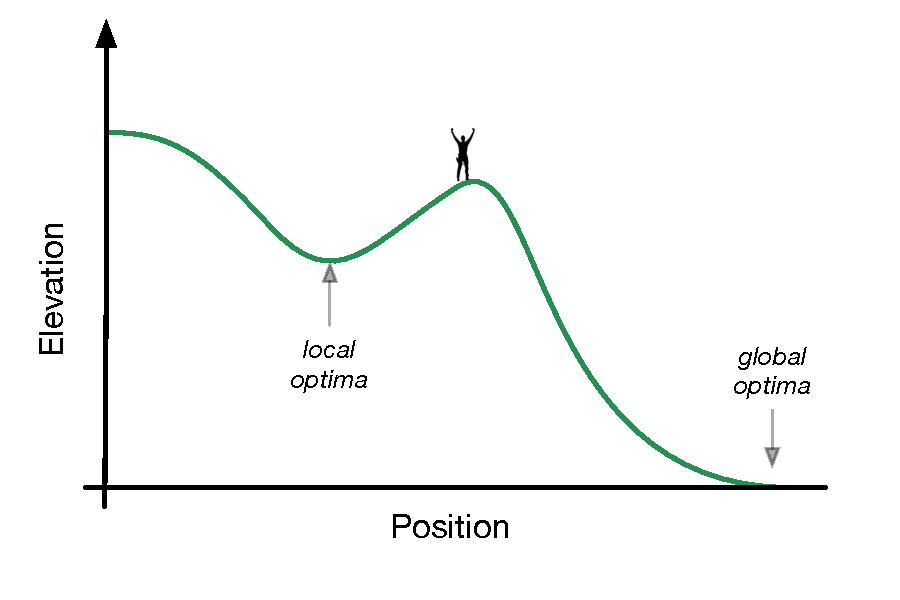
\includegraphics[width=0.6\textwidth]{descent}
\caption{Hill-climbing analogy of gradient descent.}
\label{fig:climbing}
\end{centering}
\end{figure}

% Gradient methods, a fighting chance
Gradient methods, on the other hand, exploit ``local'' improvements as a means of proceeding toward better answers.
A simple analogy helps illustrate both the intuition, and some deficiencies of the approach.
Consider the task of climbing down a hill blindfolded, illustrated in Figure \ref{fig:climbing}.
At any given time, one might poke about in every direction in an effort to find the steepest decline, and then, take a single step in the most immediately promising direction.
Eventually, save for some technical exceptions, this strategy will lead to a condition in which a locally optimal condition has been reached, i.e. any step increases elevation.
But is this the bottom of the mountain, or has our climber gotten stuck in a valley?
Thus it is an inherent difficulty of such an algorithm that it will lead to \emph{an} answer, but not necessarily the globally optimal one.
Additionally, given its greedy nature, the best step \emph{now} might not be the best step overall;
this is apparent in the diagram, where the best initial step is in the opposite direction, to the left, of the global optima, to the right.
This further illustrates the importance of initialization, and the effect that an unfortunate starting point can have on the optimization process.

Expressed more formally, the gradient descent update rule over a set of parameters, $\Theta$, is defined as its difference with the gradient of the scalar loss $\mathcal{L}$ over a set of datapoints, $\hat{D} \in D$, with respect to these parameters, weighted by a learning rate $\eta$:

\begin{equation}
\label{eq:updaterule}
\Theta_{n+1} \leftarrow \Theta_n - \eta * \frac{ \nabla \mathcal{L}(\hat{D}~|~\Theta_n)}{\nabla \Theta_n}
\end{equation}

\noindent It is apparent from this formulation that a model's ability to learn is a direct result of the estimate of the scalar loss, which depends not only on the model, its parameters, and the choice of loss function, but \emph{also} the data over which it is measured.
While early applications of gradient descent for training neural networks would compute parameter updates using the entire collection of datapoints available for training, deep learning typically leverages batch methods to approximate the overall loss.

Though the work presented here will focus exclusively on stochastic gradient descent as the numerical optimization method of choice, it is worth noting that there are alternative methods and extensions one could employ.
In addition to known issues regarding poor local minima, there are also degenerate cases in which a first-order method like this may be very slow to converge.
In practice however, gradient descent is often sufficient with some slight modifications, such as the use of slight Nesterov momentum \cite{Sutskever2013Importance}.
Alternatively, \emph{Quasi-Newton} methods compute approximations to higher order partial derivatives, which may help the optimization process recover from problematic regions in the loss surface and aid in convergence \cite{Liu1989Limited}.
These higher order methods often entail a higher computational cost, however, and it is not uncommon to employ them, or their approximations, in tandem with stochastic gradient descent \cite{Kavukcuoglu2010Learning}.


\subsection{Tricks of the Trade}
\label{subsec:tricks}

Armed with versatile complex functions and a means to automatically learn parameters, deep learning seems perfectly posed to tackle a vast array of information processing problems.
For some time however, however, only a handful of researchers were able to get positive results, thus earning it its reputation as a ``dark art.''
As with many things, the devil is truly in the details, and over time the various tricks and less principled practices necessary for success have been consolidated into a set of common strategies \cite{Bengio2012Practical}.

%   -- Tricks
\subsubsection{Penalizing Bad Behavior}

The goal of architecting a deep network is to adjust the representational power of the model to a given problem, incorporating known constraints where possible.
More often than not, however, the inherent complexity of a particular model vastly exceeds the latent complexity of the data at hand.
As a result, the learning process will result in parameter configurations that perform well on the training data, but fail to generalize to unseen data.
Conceptually, this can be understood as the model having too many options when achieving its goal state, and happening to pick one that is bad for reasons that do not factor into its objective function.
It can be said that the learning problem is under-determined, and thus additional penalties can be added to the overall loss.
Interestingly enough, this penalty-based approach is common practice in other greedy optimization systems, like capitalistic markets, where taxes and fines serve to discourage certain outcomes, e.g. dumping industrial by-products in a river.

While it is conceivable that any number of undesirable system behaviors could be quantified by some scalar measure, there are two general approaches common across deep learning.
% Weight Decay
The first, referred to as weight decay, ridge regression, or $L_2$-regularization, is classic across machine learning, and finds use in a variety of learning algorithms:

\begin{equation}
\mathcal{L}_{decay}=\sum_i\lambda~||\Theta_i||_2^2
\end{equation}

Here, the vector magnitude of the $i^{th}$ parameter, $\Theta_i$, is weighted by a hyperparameter, $\lambda_i$, summed to a scalar penalty, and added to the cumulative loss.
Conventionally, the same weight is applied to all parameters, although differently shaped parameters will bias the cumulative term.
During optimization, this has the effect of driving parameters toward, but not exactly, zero, providing an intuitive interpretation consistent with Occam's razor, i.e. prefer simpler solutions.
This often prevents the network from overfitting the training data exactly, and resulting in solutions that generalize better.

Whereas weight decay is applied to the parameters of network, \emph{sparsity} penalties are applied over intermediary representations in a network, taking the form of a cumulative weighted vector magnitude in $L_1$ space:

\begin{equation}
\mathcal{L}_{sparsity}=\sum_i\lambda~||Z_i||_1
\end{equation}

\noindent Ideally, it would be preferable to optimize the $L_0$ loss.
This problem is generally $np$-hard, however, and the $L_1$ loss, its convex envelope, serves as a differentiable approximation.
While it is not guaranteed that the solutions of each may coincide, optimizing the $L_1$ generally yields good results in practice.
As a result, this penalty will prefer sparse representations, which help \emph{disentangle} factors of variation in the data \cite{Bengio2009Learning}.


\subsubsection{Parameter Initialization}

As shown previously in the discussion of gradient descent, poor initial conditions can delay, or in some cases even prevent, an optimization algorithm from finding good solutions.
Attempts to train deep networks with error back-propagation can compound this issue, as an error signal can become insignificantly small after several layers under certain conditions.
While this is somewhat sensitive to the architectural decisions made, such as the choice of non-linearities used, all networks are sensitive to parameter initialization.

In general, sampling coefficients from appropriately tuned random distributions leads to reasonably good results.
There is little consensus on the advantages of a uniform versus normal distribution for initialization, but the primary factor to control in either case is the dynamic range or scale.
As a rule of thumb, this can be automated somewhat by using the \emph{fan-in}, or dimensionality of the input, to keep the activations of within the operating region of saturating transfer functions, i.e. sigmoid or hyperbolic tanget.
Rectified linear units, on the other hand, are far less sensitive to the choice of initialization, as half of its operating region is non-saturating, contributing to their rise in popularity.
As a result, sufficiently small, centered normal distributions, $\mathcal{N}(\mu=0, \sigma~\approx~0.01)$, work well in practice.

Alternatively, unsupervised \emph{pre-training} methods, credited with effectively jump-starting the rennaisance of deep learning, can be used to initialize networks in a data-driven manner.
Though there are different perspectives on how this can be achieved, the core concept is the same:
using a large amount of unlabeled data, train a deep network to reconstruct realistic observations in a greedy, layer-wise manner.
Then, once all layers have been initialized, conventional supervised training can be applied.
In theory, this data-driven process works by getting the parameters of the network closer to a good solution.
As mentioned previously, the first successful realization of this idea used restricted Boltzmann machines (RBMs) \cite{Hinton2006Fast}, leveraging Gibbs sampling and contrastive divergence to produce realistic samples from the model.
The deterministic variant is the autoencoder, which use data augmentation, sparsity, or weight tying to train a pair of deep, invertible functions \cite{Bengio2013Representation}.
Most recently, unsupervised pre-training has fallen out of favor somewhat, as comparable results can be obtained with rectified linear units and randomized weights, provided there is sufficient labeled data.
That said, this strategy may still prove useful for problems in which it is difficult to obtain a large amount of labeled information, such as personalized systems.


\subsubsection{Dropout}

Another recent addition to the canon of deep learning practicum is the training strategy known as \emph{dropout} \cite{Hinton2012Improving}.
As the name suggests, some percentage of parameters in a network are randomly ``dropped'' during training in estimating the loss and computing an update step.
The details of how exactly this is done vary slightly from sub-function to sub-function, but a description in terms of an affine transformation is sufficiently illustrative:

\begin{align*}
Z = f(Z | p) = \frac{1}{(1 - p)} Z \mathcal{B}(1, p)^M
\end{align*}

\noindent Here, the activations of an affine transformation, $Z$, a column vector of length $M$, are masked by a Bernoulli distribution, $\mathcal{B}$, with probability $p$.
To offset the effect of smaller magnitudes resulting from fewer units being active during training, these outputs are scaled by one minus the probability parameter, such that, in expectation over $\mathcal{B}$, the use of dropout matches the original function.
Applied in this manner, this prevents rows, or bases, in the matrix projection from contributing to the final output, inhibiting the co-adaptation of parameters.
Thus dropout is effective because the parameters are unable to depend on one another for effectiveness, and tend to learn independently good features.

Additionally, dropout has an interesting relationship with model averaging, or \emph{bagging}.
Masking parameters has the effect of selecting a subset of parameters from the given model, and therefore one of many complementary models is updated at each training iteration.
This reduces the theoretical bound on generalization error, and has been proven to greatly improve results for models prone to overfitting.


\subsubsection{Data Augmentation}

A common strategy among deep learning practitioners is to leverage domain knowledge wherever possible.
While this has an obvious connection to the architectural design and choice of loss function, another oft exploited, though less documented, opportunity is through the application of data augmentation.
The main idea here is that a collection of labeled data can be manipulated in varying degrees of realism.
This exploits the common scenario that modeling the synthesis process is typically easier than the analysis process.
While the most effective distortions are rather domain specific, common deformations include operations such as translation, scaling, additive noise, nonlinear distortion.
In this space of music, this could range from signal-level attributes, like perceptual codecs or production effects, to musically inspired augmentations, such as pitch shifting or time-stretching.


\subsubsection{Normalization}

Finally, enough cannot be said about the importance of proper data normalization.
The simplest form of data normalization is maximum scaling, such that all datapoints are bounded on the same input region.
Another form of dynamic range control is achieved by normalizing inputs to have unit magnitude in some $L_p$-space, e.g. Euclidean.
Alternatively, coefficient-wise \emph{standardization} is strongly advocated, e.g. subtract the mean and divide by standard deviation.
This can be extended via principal components analysis (PCA), which offers the added benefit of dimensionality reduction, or PCA-whitening (alternatively, ZCA), which ``whitens'' the data by scaling coefficients by their eigenvalues.
Lastly, \emph{local contrast normalization} (LCN) has proven to be a particularly useful approach to data normalization \cite{Sermanet2013Pedestrian}.
Finding inspiration from biological processes, LCN performs a form of automatic gain control over local neighborhoods, and can lead to surprisingly discriminative features even in the absence of training \cite{Kavukcuoglu2010Learning}.

% L2 constraints, bounded in volume, bounded to surface.
In addition to constraining the input space, it is also common to constrain the \emph{parameters} within a network, often taking two forms.
In some cases \cite{Hinton2012Improving}, parameters are simply constrained inside the volume of the given hypersphere, such that any time parameters are updated to values that result in a magnitude larger than 1, they are rescaled.
This constraint gives parameters freedom to adapt to the nuances of the data without growing arbitrarily large to offset the contributions of small weights.
Bounding parameters shares a loose connection to weight decay, in parameters are prevented from growing arbitrarily large, without the need for additional penalties or hyperparameters.
Alternatively, there are also successful instances of weights being constrained to the surface of the $L_2$ hypersphere, a common approach in various forms of sparse coding.


\section{Summary}
\label{sec:deep_summary}

% Origins
Building upon formal logic and biological analogy, neural networks were devised in the 1960s as an approach to information processing.
However, after initial promise, they were largely met with skepticism, indifference, or worse through the remainder of the century.
% What changed?
The few who persevered made various discoveries that, coupled with steady advances in computing technology, would eventually return neural computation to the fore:
mini-batch stochastic gradient descent made optimization computationally efficient and less susceptible to poor local minima, and encouraged further exploration of numerical optimization methods;
convolutional networks reduced model complexity and over-fitting through scale and translation invariance;
and lastly, larger labeled datasets reduced overfitting, and abundant unlabeled data could be used to better initialize networks in an unsupervised manner.

Deep learning is therefore based on two principles: first, that complex problems can be decomposed into a series of simpler subproblems; and second, what exactly these simpler subproblems are or should be can be discovered from a corpus of data.
